\documentclass{beamer}
\usetheme{Singapore}
\usecolortheme{beaver}

\title{Helion}
\subtitle{Fúzió más megközelítése}
\author{Péter Bence Gábor\\X89O8X}
\institute{Széchenyi István Egyetem}
\date{2023. Május 9.}

\begin{document}
\titlepage

\section{Bevezetés}
\subsection{Fúzió}
\subsection{Tokamak}

\section{Helion}
\subsection{Felépítés}
\subsection{Üzemanyag felhasználása}
\subsection{Üzemanyag előállítása}
\subsection{Energia kinyerése}

\begin{frame}
    \frametitle{Tartalom}
    \tableofcontents
\end{frame}

\begin{frame}
    \frametitle{Bevezetés}
    \begin{figure}
        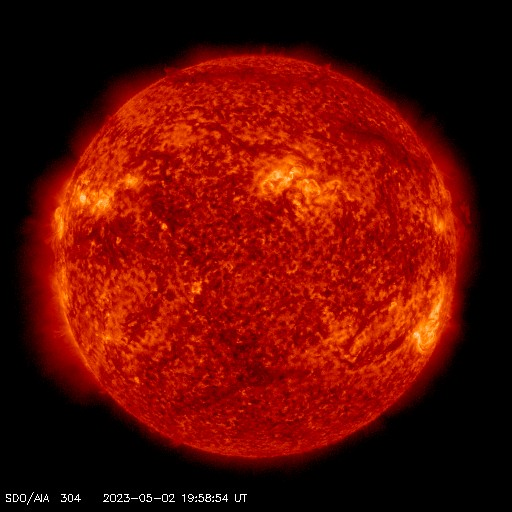
\includegraphics[scale=0.30]{latest_512_0304.jpg}
        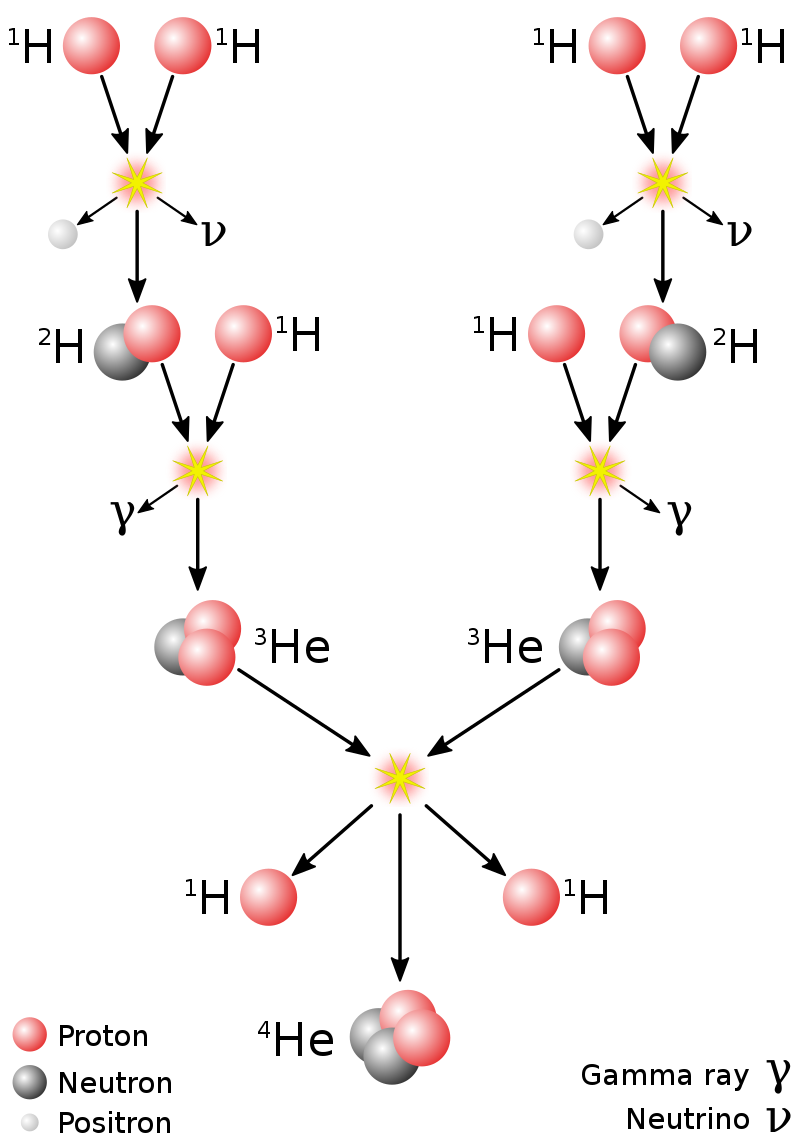
\includegraphics[scale=0.13]{800px-Fusion_in_the_Sun.svg.png}
    \end{figure} 
\end{frame}
\begin{frame}
    \frametitle{Fúzió}
    \begin{figure}
        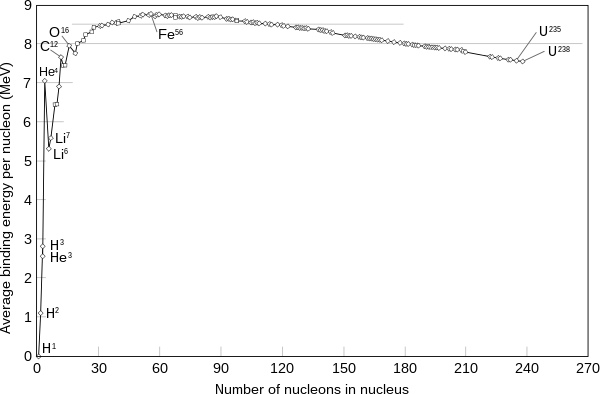
\includegraphics[scale=0.5]{Binding_energy_curve_-_common_isotopes.svg.png}
    \end{figure} 
\end{frame}
\begin{frame}
    \frametitle{Tokamak}
    \begin{figure}
        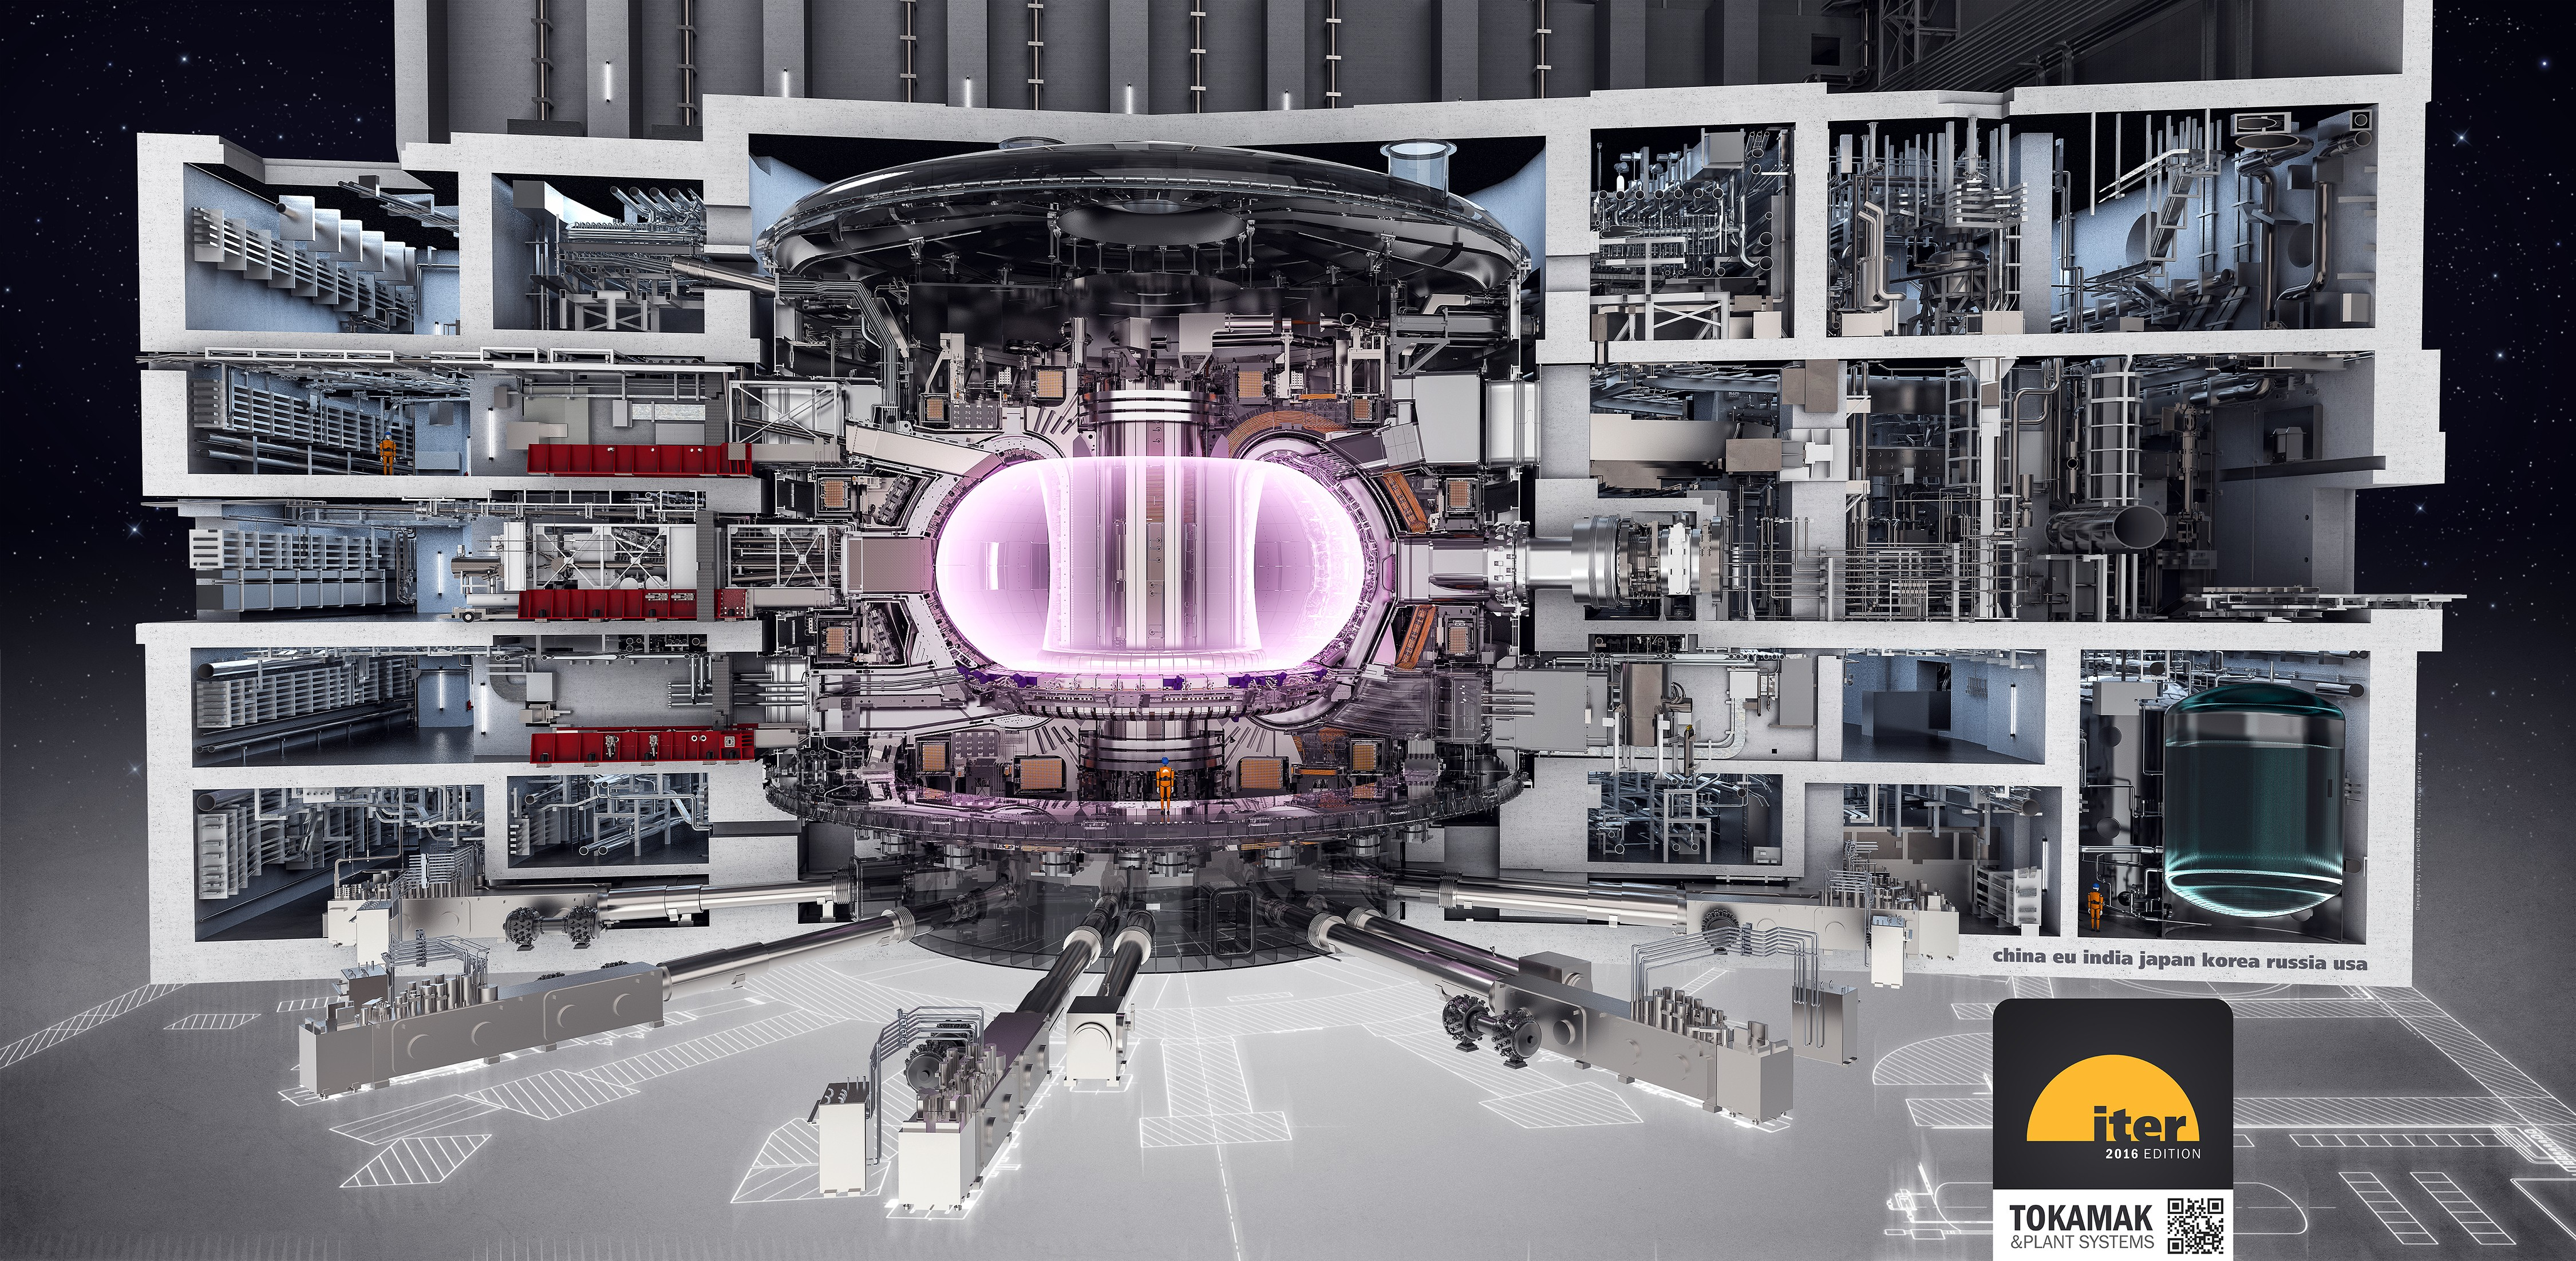
\includegraphics[scale=0.045]{iter.jpeg}
        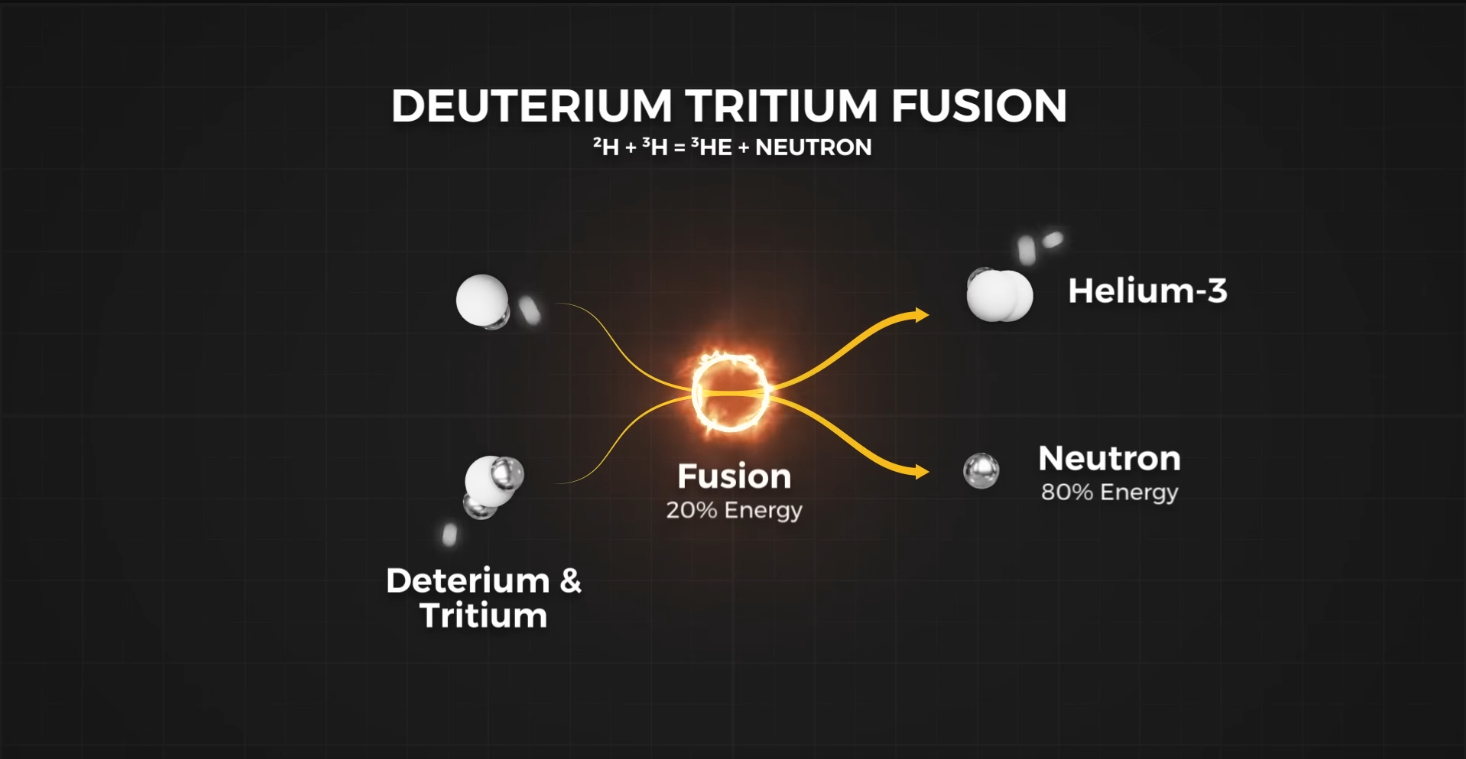
\includegraphics[scale=0.14]{deut_trit_v2.png}
    \end{figure} 
\end{frame}

\end{document}